%File: formatting-instruction.tex
\documentclass[letterpaper]{article}
\usepackage{aaai}
\usepackage{times}
\usepackage{helvet}
\usepackage{courier}
\usepackage{graphicx}
\frenchspacing
\setlength{\pdfpagewidth}{8.5in}
\setlength{\pdfpageheight}{11in}
\pdfinfo{
/Title (Insert Your Title Here)
/Author (Put All Your Authors Here, Separated by Commas)}
\setcounter{secnumdepth}{0}  
 \begin{document}
% The file aaai.sty is the style file for AAAI Press 
% proceedings, working notes, and technical reports.
%
\title{Learning augmented planning for challenging multi-agent envronments}
\author{Charles Higgins, Odinaldo Rodrigues,  Michael Luck\\
Kings College London\\
Center for Doctoral Training in Safe and Trusted AI
}
\maketitle
\begin{abstract}
Recent success in game-playing AI have relied on the combination of model-free and model-based forms of learning and reasoning respectively. This work suggests a development of the learning-augmented search which tailors the search depending on the perceived types of opponent. We provide experimental results showing it to be more robust to uncertain conditions and multiple opponent types against state-of-the art baselines. This work, we argue is among to first line of which which effectively extends reinforcement learning augmented search to larger and more complex environments
. 
\end{abstract}
\section{Introduction}
% \begin{itemize}
%     \item Opponent modelling roughly aims to compute a model of other agents in order to optimize action selection.
%     \item While a well developed field, methods have yet to extend to open environments. 
%     \item For an open environment, methods need to be swift, scalable and robust. 
%     \item This document looks at the swift component --- in short, RL agents are swift to execute, however take a while to train and can be unpredictable when dynamics shift drastically from training. Model-based reasoning approaches (planning) tends to be safer and predictable, but slow to execute. 
%     \item This document briefly discusses the state of the art in combining search and learning, and identifies gaps in the literature. 
% \end{itemize} 

It is a truth universally acknowledged that a machine-learning agent in possession of sufficient data must be in want of converging to optimal rewards. However, given a non-stationary environment, such convergence is often not possible. Any environment where the relationship between state and optimal actions change over time is deemed non-stationary, hence, any open environment where other agents might enter or leave, or learn and update their policies in response to stimuli is deemed non-stationary. 
\newline \newline
Despite prodigious advances in recent years in games posing challenges through enormous state-spaces, requiring strategic thinking and planning, multi-agent systems pose a number of open questions. Crucially, a number of these problems revolve around safe and trustworthy action-selection: in short, how can an autonomous agent act in a way a human might trust? If an agent is in a non-stationary environment, an agent cannot be sure of the results of its action before making it, and hence, cannot reasonably act safely. In the pursuit of safe and trusted AI therefore methods to address this non-stationary are required. 
\newline \newline
One assumption one can reasonably make is that the non-stationary element of a multi-agent environment is (for the most part) due to other agents, as opposed to an intrinsic part of the wider world. One can then combine a model of another agent, designed to capture the non-stationary component of the environment, with a distinct (and stationary) environment model. Hence, an agent can control, or at the very least limit the negative effects of non-stationarity, and act with increasing certainty. This is the fundamental assumption made by a group of methods which are loosely referred to as opponent modelling. Opponent modelling methods construct a distinct internal model of other agents, and use this model in to adapt their actions to this other agent. 
\newline \newline
Opponent modelling, particularly within the area of game-playing AI, has had notable successes in closed environments, however solutions have yet to extend conclusively to open environments \cite{Albrecht_stone_2019}. In order to combat some of the challenges posed by openness, an agent must learn not only to adapt to large numbers of opponents, but an agent must be able to perform opponent modelling \textit{swiftly} and \textit{robustly}: it must be able to swiftly reason over the nature of another agent (i.e. its intentions/reward function, observations, and likely actions) and, equally swiftly, use this information to act safely, and ideally, optimally. 
\newline \newline
Traditional or regular methods of action selection for intelligent agents tend to fall into one of two distinct camps: the reasoning or learning approach. The reasoning approach tends to conform to a state-space search style approach, and so fails to perform well in large or dynamic environments. In contrast, model-free learning agents tend to perform well in complex environments, however require a large training time (i.e. they have a low degree of sample-efficiency). Both therefore have significant flaws, and therefore neither are able to meet the criteria of a swift and robust agent (N.B. this line of reasoning is further explained in Section \ref{Background}). 
\newline \newline
To meet this objective: contributing a trustworthy method of action selection which is swift and robust, we propose a multi-agent extension of a Partially Observable Monte Carlo Planning agent architecture (POMCP). A POMCP agent is a model-based agent which uses an internal model of the environment to select actions which is capable of performing in large uncertain environments. We augment this architecture with an opponent-weighted policy-augmented search component. Our contribution builds upon the state of the art in opponent modelling and game-playing AI, and integrates a data-driven learning component within a model-based reasoning agent architecture. It proves to outperform both purely model-based and model-free counterparts as well as other state of the art baseline methods, given an uncertain  ad-hoc coordination environment (i hope...). To the best of the author's knowledge, this is the first hybrid data-driven/model-based system to have been applied to an opponent modelling task. 
\newline \newline
The remainder of this paper is structured as follows: Section \ref{Background} introduces the background theory for opponent modelling, data-driven action-selection in game-playing AI and reasoning approaches. 
Section \ref{MDP/POMDP} formalises the system. 
Section \ref{Contribution}introduces our contribution
Section \ref{Experiments}lists the upcoming experiments and expected results, 
Section \ref{Conclusion} concludes. 
\section{Background}\label{Background}
This section provides an introduction to various basic concepts and intuitions required to understand the contex and contribution of this line of work. It starts with an introduction into multi-agent environments and opponent modelling, before discussing various methods of action-selection and their associated benefits and weaknesses, before finally introducing the core algorithms upon which this piece of works builds. 

\subsection{Open environments \& opponent modelling}
As mentioned in Section 1, if the environment is stationary -- that is, the relationship between the state of the environment and the eventual rewards, is fixed, a learning agent can eventually learn an optimal policy: a mapping between state and actions, which maximises discounted future rewards. 
Hence, given enough data, an agent can learn to act optimally, and therefore safely, in such environments. However when the relationship between state and optimal actions change, converging to an optimal policy is not theoretically posisble. This however poses a problem as in reality, most environments exhibit a degree of non-stationarity. Indeed, a great number of these environments, non-stationarity comes as a result of other agents. Take for example, the challenge of an autonomous vehicle navigating down a coridoor. 
\newline \newline
In a single-agent environment, there is a simple optimal policy. Given enough iterations, an agent can learn how best to optimise actions to eventually move (in as few moves as possible) towards the exit. 
\newline \newline
Indeed even given a more complex relationship between optimal action selection and state, like partial observability, or noisy movements (i.e. the relationship between state-action pairs and the sucessive state is probabilistic), the optimal policy should adjust, and will remain fixed. Mathematically speaking, this environment exhibits the markov-property, where firstly, there exists an optimal policy, and secondly, the optimal policy is inferrable from only the current state (i.e. memoryless).
\newline \newline
Consider now, the same environment, but there exists at least one other agent. The optimal policy now depends on the state of the environment and the position of the other agent. Now,reasonably, one could image the other agent as being included in the state --- and indeed, if the other agent has a fixed policy, the envinronment is still stationary, however if that other agent learns, or updates it's policy, or enters and leaves, the environment is fundamentally changing...  


\subsection{Action-Selection}
In general terms there are two broad approaches to action-selection for autonomous agents: a learning vs a reasoning approach. The former starts with limited knowledge about the environment, and through sucessive trials and learning from actions and rewards, decides to learn a policy. The latter typically requies more domain knowledge, and reasons about actions before they are made in order to meet some objective/reach a desired state. 
\subsection{Learning vs Reasoning (high level)}
While this section is deliberately high-level, it makes a crucial point as to the strengths and weaknesses of data-driven learning vs reasoning approaches. 
In general, data-driven approaches can perform well, given sufficent time and resources to learn an optimal policy within a stationary environment. This policy often takes a huge amount of time to learn and develop as the agent learns the effects its actions have upon the environment. However, once learned, typically the execution is very swift --- depending on the exact architecture used times vary --- usually a single look-up in a Q table, or a single forward pass through a neural network. They also require very little expert knowledge to impliment, and given a stationary environment, can learn an optimal policy to maximise rewards. 
\newline \newline
In contrast, the reasoning approach requires very few, if any, learnig iterations before performing well. Rather than learning from scratch, reasoning agents typically have a model of the environment (hence the nominer model-based) which they query, testing out the likely effect of each possible action, and subsequent action. Typically, such agents are referred to as planners. These planning agents search for a chain of actions which take them from their initial state to a percieved goal state. As the search space expands exponentially in the number of sequential actions, this search is costly, and hence, at run time, these agents tend to be very slow. 
\newline\newline
In designing a swift agent therefore, one would require the intial performance of a reasoning agent, however the low-latency and swift response of a learning/data-driven agent. 
\newline \newline
One must also address the concept of robustness, and so the consequential qualities of safety (and subsequent trust, or lack thereof): data-driven or learning agents are hard to predict --- should the environment differ from that of their training, performance degrades significantly. 
Further, such are prone to unpredictable and inexplicable action-selection, limiting their applicability from fields which contain any real element of risk. In contrast, reasoning agents are often deemed 'safer'. 
They typically adapt well to changing circumstances, as their internal model already captures some of the environment's dymanics. 
Furthermore, as such agents they investigate the results of each action before they undertake it, given the assumption that their comprehension of the environment dynamics is correct, they act safely and robustly.



\subsection{Reinforcement learning augmented search} \label{RL + Search}
In recent years, the combination of model-based search methods and deep reinforcement learning (via self-play) has achieved super-human performance in a number of benchmark challenges in game playing (adversarial) AI \cite{AlphaGo,Brown2020,Lerer2019}. 
The major difficulties of these domains (Chess, Go, even Poker) is that of a truly enourmous state-space. Research which has acheived noteriety has combined local state-space search with deep neural networks to approximate complex functions. 
\newline \newline
While each of the mentioned papers contribute different novel features, the basic structure of these algorithms remains constant: a sample-based search algorithm augmented with two learning components, commonly referred to as a value network, and a policy network respectively.
\newline \newline
Briefly, these algorithms structure the environment as an extensive form game (a search tree). Nodes represent states, and actions represent transitions from one state to another. Given a simple environment, a planning algorithm can search through the possible states, and select the optimal action in order to maximise rewards. However, given a complex environment, the possible state-space expands exponentially, swiftly rendering a typical search-based solution intractible. To address the issue of an enourmous search space, a \textit{sample-based} search algorithm is employed. 
\newline \newline
A sample based search algorithm constructs a search tree of immediately reachable states (rather than all possible states), given available actions. As there are a huge number of possible sequences of actions, rather than exhaustively searching the entire search-space, a sample-based search tree expands and samples only some branches (possible options), and averages across the expected rewards of immediate actions to select the best action at a given node in the tree at a given time.
\newline \newline
Even with a sampling-based approach, the seach space is often still prohibitively large, and so data-driven learning methods can be used to restrict the search space further to improve performance. Two distinct learning components (deep neural netowrks) are typically employed.  
\newline \newline 
Both networks are trained through a combination of supervised learning and reinforcement learning via self-play (playing oneself). At run-time, the policy network guides the search through the search tree (limiting the branching factor from areas of the state-space which are unlikely/unfavourable). The value network truncates the depth of the search tree by approximating the value (i.e. the expected discounted reward achievable) for a given state. In short, the learning parameters allow for a tractable approximation of vast state-space, while allowing for explicit reasoning over the short-term, or immediate search-space. 
\newline \newline
While arguably the most famous result was DeepMind's Go-playing AI AlphaGo \cite{AlphaGo}, which rather dramatically defeated Lee Sidol, both Chess and Go are perfect information games --- the state of the game is certain and visible at all times. In a development of earlier Poker-playing bots, Brown et al. \cite{Brown2020} tackled the problem of imperfect information games (namely head's up no limit texas hold 'em poker) by adapting the notion of state to a public-belief state. In short, they define a mechanism for transforming an imperfect information game into a continuous state-space perfect information game, where the state contains a probabilistic distribution over all agents beliefs (a public-belief state). Through this transformation, a similar algorithm to Silver et al's AlphaGo can be used, with policy and value networks guiding and truncating search.   
\newline \newline
Crucially, this research approaches the problem of large state-spaces rather more from the side of learning as opposed to reasoning. In contrast, a body of work has tackled partially observable environments with an explicit focus on reasoning: planning.  


\subsection{(Sample-based) Planning}
 Planning is, in essence, a search problem --- an agent queries an internal model which captures the dynamics of the environment to find a sequence of actions to achieve some goal state or maximise a reward. In complex domains, the search-space swiftly becomes so large as to be computationally intractable, hence the recent focus on model-free forms of learning to solve similar problems. However, model-free approaches tend to be unpredictable. As they have no model to reason about the environment, they can exhibit incorrect and even dangerous behaviour in unforeseen scenarios --- typically there is no reasoning process, but simply a mapping of a state to an action. Given this unpredictability, the application of purely model-free approaches to some domains carries risk and is therefore undesirable. Extending planning to complex domains remains an open question and a valuable and viable direction of enquiry. At present, the most promising area appears to be sample-based planning, which requires exploring only some of the search space online (i.e. at runtime).  

\subsubsection{Monte Carlo Tree Search --- an approach to search in a large state-space}
Monte Carlo Tree Search is a sample-based search algorithm which requires a simulation model of the environment to evaluate possible actions and future states in order to converge to an optimal policy online (i.e. re-evaluating from each state). 
Each node represents a possible state, and transitions (edges) are possible (probabilistic) actions. At a given state, an agent traverses a computed tree, selecting actions with a heuristic until reaching a leaf node. At the leaf node, it then randomly selects actions and receives a potential successor state from the transition model. This is referred to as a rollout, and continues to some arbitrary depth of tree depending on available resources. It then evaluates the state and the rewards achieved in the leaf node, and propagates the rewards backwards up the tree. This cycle  (traversal, simulation (rollout) and backpropagation) then continues for a determined period, until a new action is selected, and a new state observed. 
\newline \newline
This sampling-based approach is typically paired with a UCB1 algorithm (upper confidence bounds) which balances exploitable actions with under-explored alternatives, which has shown to converge (eventually) to an optimal policy \cite{Ross2011}. 
\newline \newline
This approach, typically when paired with a strong heuristic and an accurate transition/environment simulator, has shown to be an effective and powerful approach to action-selection in complex environments with large search spaces --- this algorithm forms the basis for most of the recent successes in adversarial AI (as described in the previous Section: Section \ref{RL + Search}) 


\subsubsection{Monte Carlo Search in a partially observable environment --- adopting MCTS to partially observable environments}
Despite the success of a sample-based approach, the extension of planning to uncertain (partially observable) environments still poses problems. 
In such an environemt (due to inperfect or incomplete observations), an agent is (initially) uncertain of the actual state. This casuses considerable complexity, and has ramifications for the time and space requirements for computing an optimal policy.
In an $n$-stateful environment, an agent must compute a distribution over $n$ states representing its belief over the true state of the environment. 
It must compute this in addition to the generic planning complexities of all possible actions, transitions and resulting states --- hence unless facing a very trivial problem in an exceedingly simple environment, the exponential complexity of partially observable environments tend to render planners inapplicable. 
\newline \newline
Silver and Veness  \cite{Silver2010} combined a sampling-based approach to belief updating (particle-filtering) with a monte-carlo tree search style algorithm which allows for partially observable planning. Among a number of alterations, each node in the tree is based on an observation history rather than a state, reflecting the agents belief over the state. In effect, Monte Carlo methods are used in a bi-directional manner: forwards to evaluate action selection; backwards to update belief over states. 
\newline \newline
In small state spaces, the belief-state (i.e. distribution over the possible state) can be perfectly calculated by applying Bayes rule --- in large state spaces this can be computationally demanding, and a compact representation of the transition model (in terms of likelhihoods) might not be available. To address this problem Silver and Veness contributed an algorithm, Partially Observable Monte Carlo Planning (POMCP), which uses a particle-filter: generating a number of small unweighted particles, each representing a possible state, and evaluating them based on expected vs received observations. They use this sampling-based approach to update the belief about the likely history at each time-step, and iteratively converge onto the true state.
\newline \newline
As with typical Monte Carlo methods, the sampling approach greatly limits the search space as only (likely) reachable states are evaluated, and the belief over states can be efficiently computed. In short, sampling based methods have shown to allow for swift approximation over complex belief spaces.

\subsubsection{Improving on POMCP --- updating the environment simulation}  
Despite the theoretical success of POMCP, belief-based planning still poses challenges. 
While known for its efficacy in dealing with large state-spaces, MCTS is limited by the accuracy of the transition model. Simply put, if the model of the environment provided to the planner is not sufficiently expressive as to capture the environment dynamics, despite efficient sampling, the performance of an agent will be poor. 
\newline \newline
In recent years, there have been two notable works which have augmented belief-based planners with a learning capacity in order to overcome an incorrectly specified model. 
\newline \newline
Katt et al \cite{Katt2017} augmented the notation of a POMDP to take account of a number of extra features, to allow for a Bayesian updating of the environment model --- in effect the transition dynamics were updated as experience increased in a Bayesian way, allowing for more realistic rollouts and better action selection. In short, they incorportated a learning element into the model of the environment to allow for an incorrectly or incomplete black-box environment simulation. 
\newline \newline
With a similar aim, Hayashi et al \cite{Hayashi_et_al2020} augmented a POMCP planner with a deep-recurrent neural network as a mechanism for particle reinvigoration (suggesting possible states to evaluate), which suggested better candidate states (particles) to be computed allowing noisy or incorrectly specified environments to be used without resulting in poor agent performance. They phrased the environment simulator as a black-box with various parameters which required fitting. This fitting took place as experience grew, meaning that the black-box simulator could be tuned online, allowing the world-model to be iteratively updated. Crucially, they applied this to an opponent modelling task, the level-based foraging domain \cite{Papoudakis2020,Barrett2015}, in which agent types were parameters within the black-box simulator. 

\subsubsection{Improving MCTS --- information theoretic rewards}
Finally, Fischer and Tas augmented a MCTS style of planning with information theoretic rewards in a continuous domain. This means in practice increasing an internal reward for reaching states where the agent received more information about the environment. The basic idea behind this is that often as an agent's understanding of a domain increases, the convergence to optimal action selection is swifter. While this was tested in a single-agent domain, the concept of augmenting a sampling-based search procedure with information-based rewards showed promise \cite{Fischer2020}. Despite the domain being marginally different from that of opponent modelling, the concept of explicitly rewarding an agent for looking for information has parallels in opponent exploration. Ultimately, the concept of deliberately manipulating a game state to learn more about an opponent is worthy of investigation, and seems at present somewhat under-explored.

\subsubsection{Incoporating agent models into MCTS}
As mentioned previously, a MCTS involves several stages: 1) traversing a tree via a best-first (heuristic) until reaching a leaf node; 2) Upon reaching a leaf node, it performs a rollout, which involves selecting an action, and sampling an environment simulator for a possible next state and expected reward. It continues this rollout to an arbitrary depth. 3) Finally, having reached a maximum deapth, the reward is propagated back up the tree to the root node.
\newline \newline 
In a multi-agent environment, the transition function responsible for mapping one state to another depends on a joint actions taken by all agents. Hence, in a rollout, the simulator must assume a joint action (i.e. infer/suggest likely actions taken by \textit{other} agents). In this way, agent models are integrated into a MCTS via the simulation phase. In simple terms, they are implicitly included in the environment model. In both \cite{Hayashi_et_al2020} and \cite{Albrecht_stone_2019} agent models are computed and viewed as parameters to be tuned in this environment, thus providing an interesting middle ground between a `global' approach, in which an agent simply learns a single generative model of  the environment from scratch (no opponent models), and a typical opponent modelling approach, which requires distict agent models and environment models.
\newline \newline
This method also has benefits as it translates the problem of opponent modelling into one of state-space search, allowing for the incorporation of policy/value netowrks and/or sampling-based planners to address complexities of opponent modelling, which often result in large (probabilistic) state-spaces.  
\section{Formalisation} \label{MDP/POMDP}
\subsection{Partially observable Markov Decision Process POMDP}
The environment can be phrased as a partially observable Markov decision process (POMDP). 
A POMDP is defined as a tuple: 
\begin{equation}
    \langle S, A, O, P, Z, R, \gamma, b_0 \rangle
\end{equation}

\noindent$S$ is the set of states, $A$ the set of actions, $O$ the set of observations; 
\newline \newline  
$P = Pr(s_{t+1}|s_t, a_t)$ is a stochastic transition function, mapping a state and action to ta new state. \newline \newline 
 $Z = Pr(o_{t+1}|s_{t+1},a_{t})$ is the stochastic observation function --- observations are not certain, hence the it is defined as the probability of observing a certain observation having taken an action in a given state. 
 \newline \newline
 $R = R(s_t, a_t)$ is the reward function;
 \newline \newline
 $\gamma \in [0,1]$ is the discount factor (discounting future rewards);
 \newline \newline 
 $b_0$ is the belief about the initial state.
\newline \newline 
At any time $t$, an agent takes an action ($a_t$), receives an observation ($o_t$) and reward ($r_t$). The agent aims to derive a policy $\pi$ which maximises its total discounted reward given its beliefs in a certain state. 
\newline \newline
Crucial to efficient planning and action selection is to minimise or eliminate the mismatch between the agent's belief/encoded model of the environment and the dynamics of the real environment (i.e. the ground truth). This model of the environment is expressed (in this framework) by the observation (imperfect observability) and transition functions. 
\newline \newline
To simplify, let the state-transition function be interpreted as $s_{t+1} \sim f(s_t,a_t)$, and the observation function be $o_{t+1} \sim g(s_{t+1}, a_t)$. 
\newline \newline
Given that the state can be changed by other agents, one can view the environment as having a joint action-space between the actions of an agent and all other agents present. Hence, with the assumption that another agent is present, one can then reform the state-transition function and observation functions to take into account the joint actions of all other agents and the environment dynamics, which shall be represented by $\Theta$: 
\begin{equation}
    s_{t+1} \sim f(s_t, a_t|\Theta) 
\end{equation}
\begin{equation}
    o_{t+1} \sim g(s_{t+1}, a_t|\Theta) 
\end{equation}
\newline \newline
Opponent modelling can be seen as an attempt to improve this model $\Theta$, by explicitly modelling an opponent, or group of opponents. 
The quality of the model dictates the quality of the state-transition and observation functions, and therefore the quality of the overall policy derived. 
\newline \newline
One can view $\Theta$ as an encapsulated opponent model, which when fed to a black box environment simulation (the function $ f(s_t, a_t|\Theta$) provides a projected next state.
\newline \newline
By way of an example, an agent would enter an environment with a belief over the likely parameter(s) of $\Theta$. As interactions continue, an agent can update the value(s) of $\Theta$ based on observations: the values of $\Theta$ are not immediately obvious however they can be inferred from observations/prior knowledge and some form of reasoning. Hence, the belief of an agent at time t can be seen as a joint distribution over:
\begin{equation}
    b_t(s,\Theta) = Pr(s_t,\Theta | h_t)
\end{equation}
where $h_t$ is the history of observations and action pairs ($h_t = [a_0, o_0, a_1, o_1 ... a_{t-1}, o_{t-1}]$) taken to reach the state $s_t$. In other words, the opponent model is included in an uncertain state-representation. Hence, in reasoning over the state, the agent also reasons over possible opponent models given an action history. 

\subsection{Parameterisation of $\Theta$} \label{IncludingAgentModels}
The previous section provides a general framework of simulation-based action-selection which makes use of an internal agent model to better inform an observation and state-transition function. This serves to show how an opponent model might fit into the action-selection pipeline.
\newline \newline
The definition of $\Theta$, and methods to accurately estimate $\Theta$, where theta refers to an number of opponent models in an open environment is completed by a simulation based component known as a particle simulator (this is explained further in section TODO:INSERT SECTION).
\newline\newline
In the simplest form, $\Theta$ refers to a vector containing agent models: ${\theta_0, \theta_1,...,\theta_n} \in \Theta$. 
\subsection{Type-based reasoning}
Each $\theta_i \in \Theta$ is an agent present in the environment.    
\subsubsection{Type-based reasoning}
A popular and swift method of opponent modelling is type-based reasoning. Rather than building an assumed policy from scratch at run time, a modelling agent assigns a pre-specified agent model to an observed agent. This has often been supplied by the user, or (recently) has been learned over repeated interactions with other (similar) agents. 
This leads to a (potentially) large number of agent \textit{types}: $\phi \in \Phi$.
\newline \newline
Hence, the parameter of $\phi$ in $\theta_i$ refers to agent model $\theta_i$ as being of type $\phi$. 
\newline \newline
Hence, in terms of the belief updating, one can rewrite the belief over state and model parameters, given an observation history to the belief over state and type of model, given an observation history. 
\begin{equation}
    b_t(s,\Theta) = Pr(s_t,\theta_i = \phi | h_t)
\end{equation}




  
\section{The building blocks: basic algorithms}
The following section defines the basic methods upon which the contribution builds. It begins by describing a weighted particle filter for probabilistic state-estimation, a Monte Carlo Search Tree, and finally describes the architecture of a (modified) Multi-Agent Partially Observable Monte Carlo Planner \cite{Hayashi_et_al2020,Silver2010}.  
\subsection{Particle Filtering: iterative approximate Bayesian Updates}\label{ParticleFiter}
Traditionally the use of Bayes Law is used iteratively in each timestep to reason over uncertain information to update the posterior probability of being in a certain state.
\begin{equation}
    b_{t+1}(s') = \frac{O^{s' a_t z_{t+1}} \Sigma_{s \in S} P^{s a_t s'} b_t (s)}{\Sigma_{s'' \in S} O^{s'' a_t z_{t+1}}  \Sigma_{s \in S} P^{s a_t s''} b_t (s)}
\end{equation} 
% This shows the computation necessary: the belief update over the state is equal to the probability of recieving an observation in state $s'$ given the previous action and observation. This is multiplied by summing over the transition probabilities of taking an action in the previous state, given the previous belief state. Finally this is all normalised over the sum over all possible states of the observation of reciving this observation, given the previous state and action if not in state $s'$ multiplies by the sum over the transition probabilies of moving from the previous state having taken action $a_t$ and arriving in not state $s'$ multiplied by the previous beliefs.
\newline \newline
In complex environments (particularly those where there are multiple opponents), performing a complete Bayesian update can be so costly as to be intractable. Hence, recent works in opponent modelling have used deep-learning to approximate the update (see for example \cite{he_om_DRL}). However deep-neural nets require training, and can take many iterations before being successful. A recent strategy for opponent modelling (adapted by \cite{Hayashi_et_al2020}), however proposed to expand Monte-Carlo planning to partially observable domains is a sampling based approach which makes use of a generative environment model. This environment model ($G$) can be used to perform Bayesian Filtering. 
\newline \newline
The belief state (i.e. the belief distribution over possible states) is sampled for a history $h_t$ by $K$ particles, with index $i$ and a weighting of $w$ 
\begin{equation}
    k \in K, k = \langle i, w \rangle; B^i_t \in S, 1 < i < K    
\end{equation}
Each sample represents a possible state, and the belief-state is the weighted sum over all particles. 
\newline \newline
Particles are iteratively removed and reinvigorated at each timestep. At the start of a game/iteration, K particles are sampled from the initial belief-state. The agent selections an action $a_{t, real} \in A$, and receives an observation $o_{t+1,real}$. 
\newline \newline
Each particle is then evaluated. From the state in $K$, an agent uses the internal generative model to provide a sample of a successor observation: 
\begin{equation}
    o_{t+1, possible} = G(k_i, a_t)
\end{equation}
This possible state is then compared to the real observation via a distance metric to return a value of the accuracy of this particle $V(k)$, which in turn is used to update the value of each particles weighting ($w_k$) (by a learning rate denoted $\gamma$) 
\begin{equation}
    V(k_i) = o_{t+1, possible} - o_{t+1, real}
\end{equation}
\begin{equation}
    w_{k_i} \leftarrow w_k + (- \gamma * V(k_i))
\end{equation}
The weaker particles are pruned based on a hyperparameter depending on the relative strength of weightings. Finally, new particles are created by sampling and adding Gaussian noise to existing particles. 
\newline \newline
The result is that as the history increases (i.e. more observations are evaluated) the belief-state should converge as inaccurate state hypotheses are filtered, and more accurate hypotheses increasingly suggested. 

\subsection{Monte Carlo Tree Search --- an approach to search in a large state-space}\label{MCTSDesc}
Monte Carlo Tree Search is a sample-based search algorithm. 
Similar to a particle filter, it requires a generative model of the environment ($G$) to evaluate possible actions and future states in order to converge to an optimal policy online (i.e. re-evaluating from each state). 
\newline \newline
An agent begins in a state ($s_0 \in S$). From this state, it constructs a sample-based search tree of possible successor states.
\begin{equation}
    T \sim \langle N, E \rangle
\end{equation} 
\begin{equation}
    N \sim \langle s, q, v \rangle 
\end{equation}

In this search tree, each node ($n \in N$) represents a possible state ($s \in S$), and transitions (edges ($e \in E$) are possible (probabilistic) actions, mapping a node to a probable successor node given a state and action pair. 
\newline \newline
In each iteration, the tree is traversed in a best-first search procedure. Typically, the value of selecting a node is estimated by the upper-confidence trees algorithm (an adapted upper confidence bound UCB1 bandit algorithm). This weights the relative value of the explored node with an exploration value (derived by the expression on the far right of equation \ref{UCB1}) which weights the number of times that node has been explored relative to its parent node, by the scalar constant $c$ (which typically takes the value of 2).
\begin{equation}\label{UCB1}
    V(n \in N) = V(n) + c \sqrt{\frac{log(parent(n)_{visits})}{n_{visits}}} 
\end{equation}
Given a sufficiently large tree, this approach has shown to converge (eventually) to an optimal policy \cite{Ross2011}. 
Having reached a leaf node (i.e. a node in the tree $T$ with no children), children are generated by \textit{expanding} the node. In this case, all possible successor states of the node are created and added to the tree by use of the generative environment model $G$. 
\begin{equation}
    s_{t+1, possible} \leftarrow G(s_t, a_t)
\end{equation}
Having generated the successor states, the agent estimates the value of each state by performing random \textit{rollouts} to a predetermined depth. These \textit{simulations} (sometimes referred to as \textit{rollouts}) take the form of a random sequence of actions, and return the rewards for the successive states. The reward of potential future states are sampled from these rollouts by taking the mean eventual reward for a single starting state. For $x$ number of rollouts:
\begin{equation}
    Q(n \in N) = \frac{1}{x}\Sigma_{i=0}^x R^i
\end{equation} 
where $R^i$ is the reward over the $i^{th}$ rollout.
\newline\newline
Finally, the estimated values of the leaf nodes are backpropagated throughout the tree, in order to allow for potential future states to add value to their parent states, until finally all the possible moves available in the initial state (the root node) have accurate values, from which one can select an optimal action. 
\newline \newline
For a fixed time-period or for a fixed number of simulations, the cycle of \textit{tree-traversal}: traversing the tree $T$; \textit{expansion}: simulating all possible actions in a given state to add all possible successor states to the tree; \textit{Simulation/rollouts}: performing random rollouts to estimate the value of the state; and \textit{backpropagation}: propagating expected rewards back up the tree. This cycle then continues for a determined period, until a new action is selected, and a new state observed. 
\newline \newline
This approach, typically when paired with a strong heuristic and an accurate transition/environment simulator, has shown to be an effective and powerful approach to action-selection in complex environments with large search spaces --- this algorithm forms the basis for most of the recent successes in adversarial AI (as described in more detail in Section \ref{RL + Search}) 

\begin{figure}
    \caption{Graphical representation of the four stages of a single iteration a Monte Carlo Tree Search, where $X$ represents the number of samples taken per timestep.}
    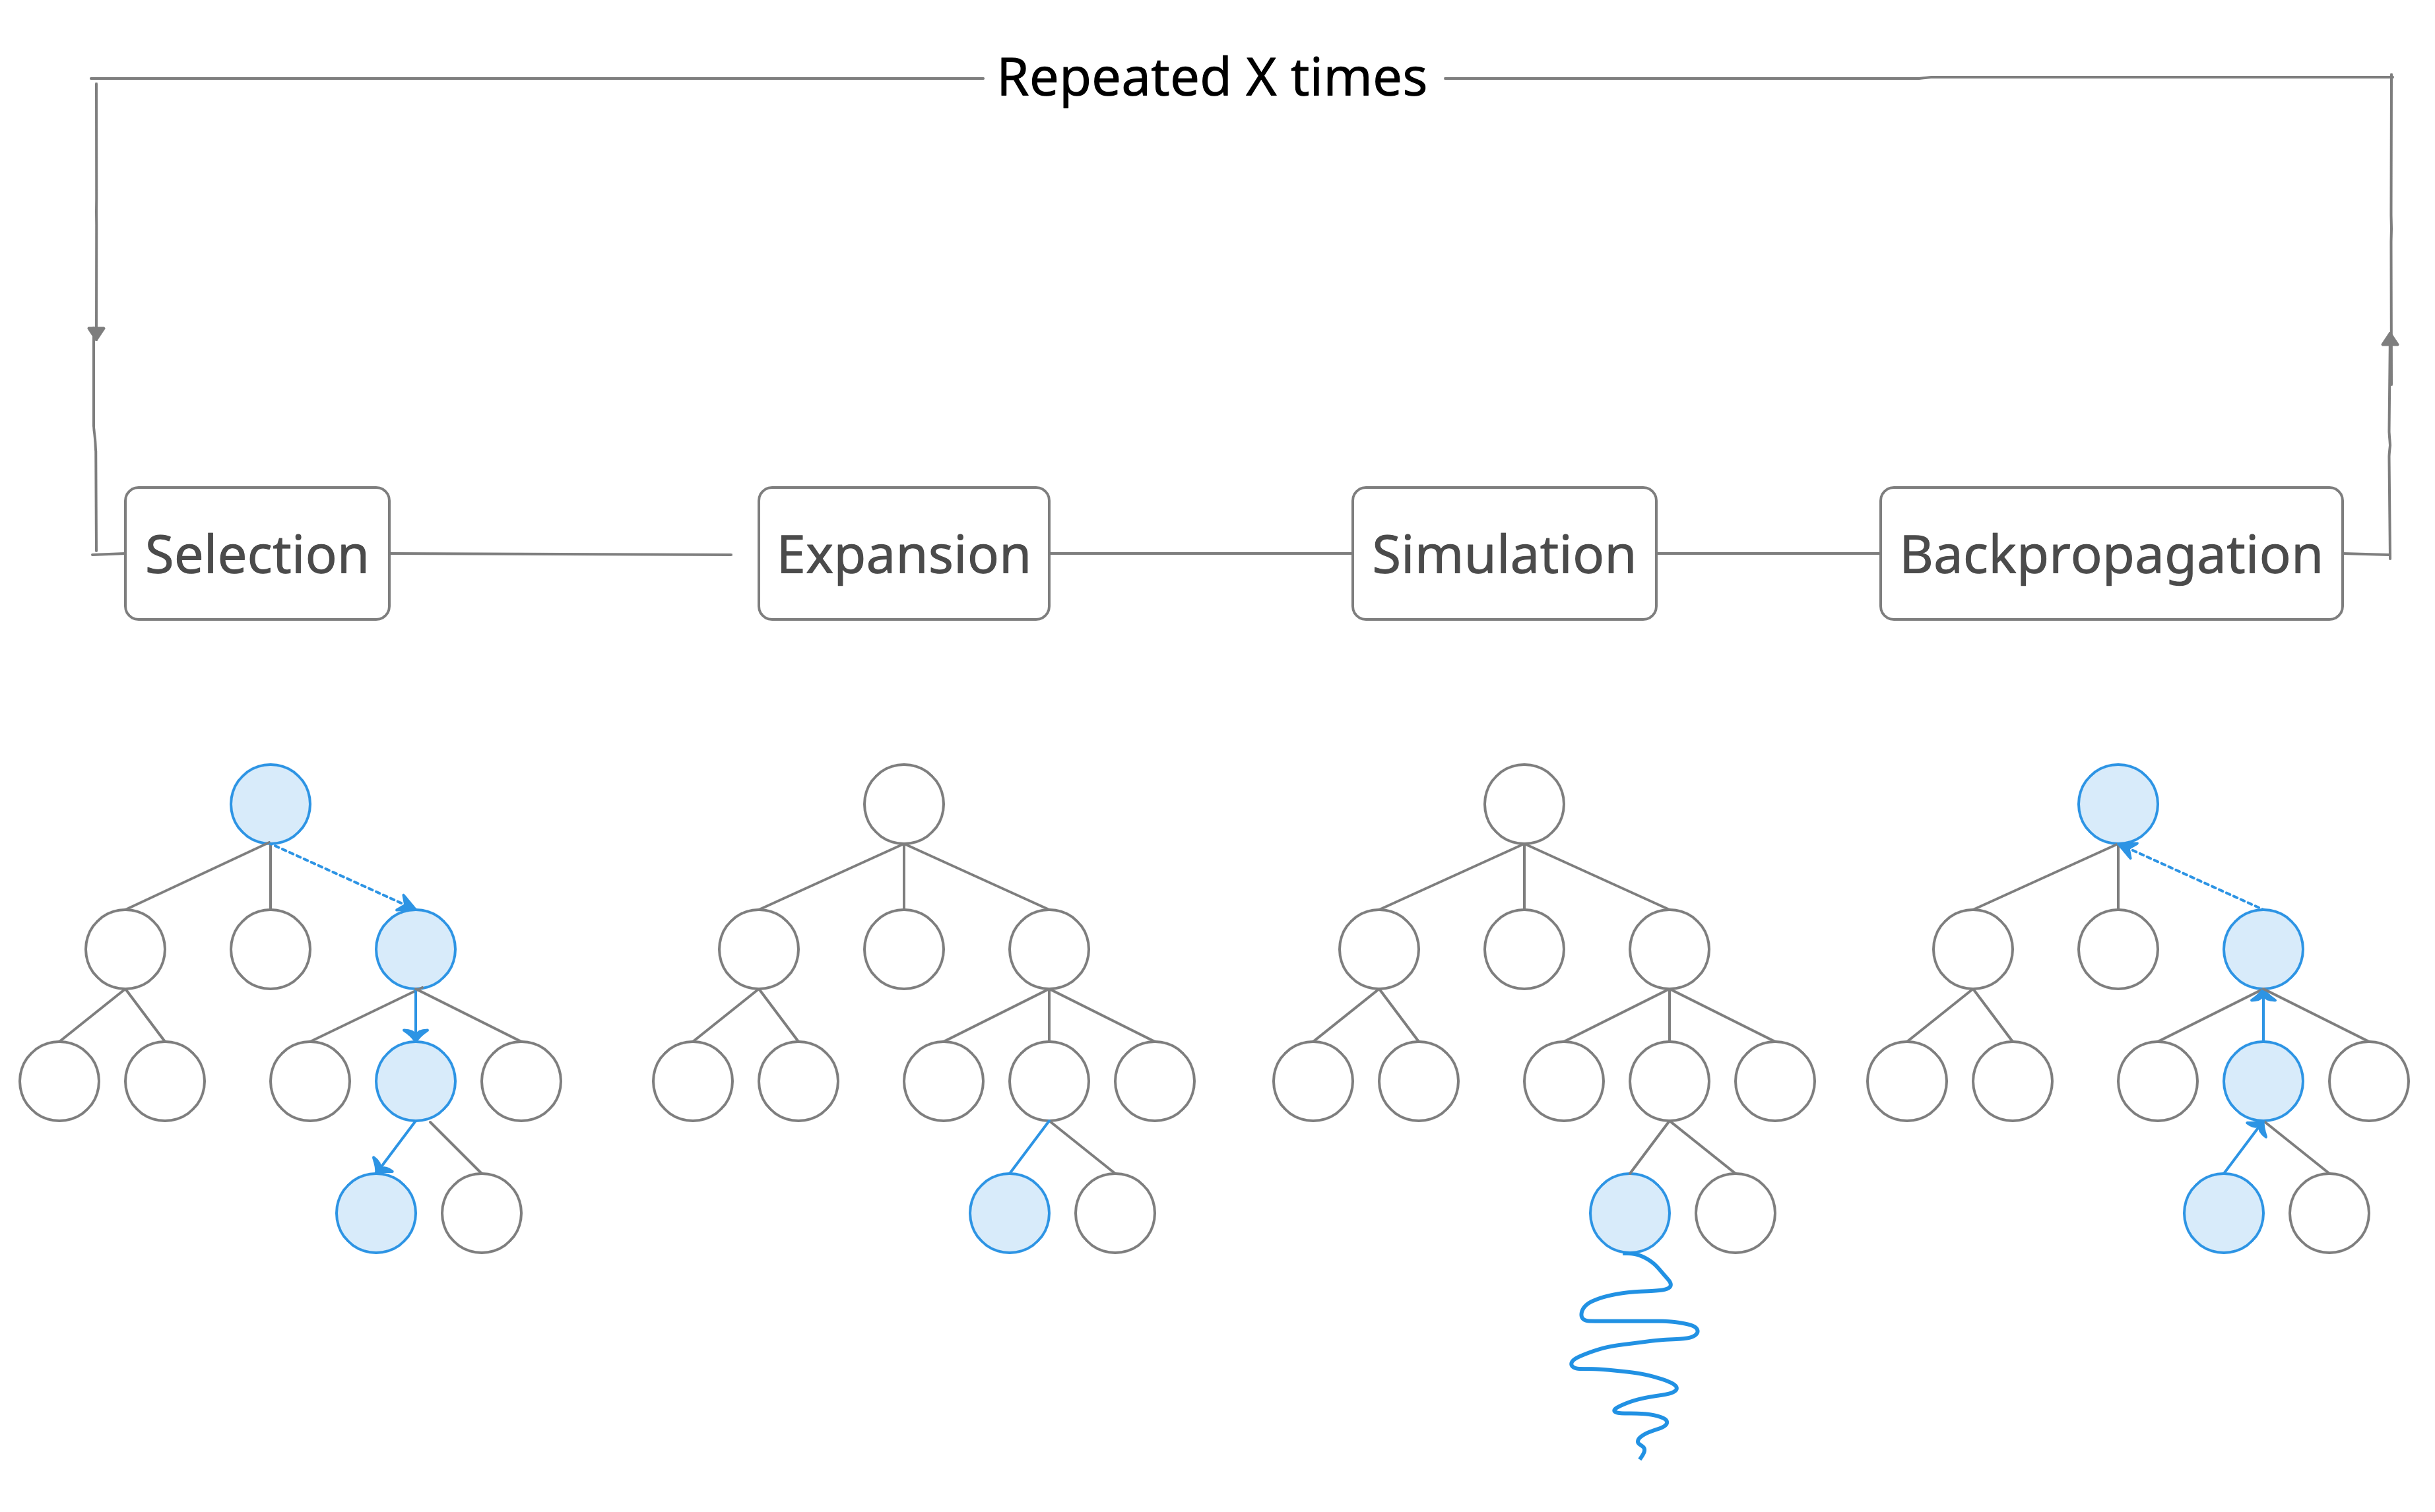
\includegraphics[width = \textwidth]{Figures/MonteCarlo.png}
    \centering
\end{figure}

\subsubsection{Aadapting Monte Carlo Tree Search to partially observable environments}
Despite the success of a sample-based approach, the extension of planning to uncertain (partially observable) environments still poses problems. 
In such an environemt (due to inperfect or incomplete observations), an agent is (initially) uncertain of the actual state. This causes considerable complexity, and has ramifications for the time and space requirements for computing an optimal policy. 
\newline \newline
In an $n$-stateful environment, an agent must compute a distribution over $n$ states representing its belief over the true state of the environment (also known as a belief-state). 
It must compute this in addition to the generic planning complexities of all possible actions, transitions and resulting states --- hence unless facing a very trivial problem in an exceedingly simple environment, the exponential complexity of partially observable environments tend to render planners inapplicable. 
\newline \newline
Silver and Veness  \cite{Silver2010} combined a sampling-based approach to belief updating (particle-filtering) with a monte-carlo tree search style algorithm which allows for partially observable planning. Among a number of alterations, each node in the tree is based on an observation history rather than a state, reflecting the agents belief over the state.  
\newline \newline
In small state spaces, the belief-state (i.e. distribution over the possible state) can be perfectly calculated by applying Bayes rule --- in large state spaces this can be computationally demanding, and a compact representation of the transition model (in terms of likelihoods) might not be available. To address this problem Silver and Veness contributed an algorithm, Partially Observable Monte Carlo Planning (POMCP), which uses a particle-filter: generating a number of small unweighted particles, each representing a possible state, and evaluating them based on expected vs received observations (as described in detail in Section \ref{ParticleFiter} and Section \ref{MCTSDesc}). They use this sampling-based approach to update the belief about the likely history at each time-step, and iteratively converge onto the true state.

\begin{figure}
    \caption{Graphical representation of the POMCP architecture: the Simulator/Generative model is used both to reason over the apparent state based on an action history, but also to reason over the best possible action absed on a sample-based planner}
    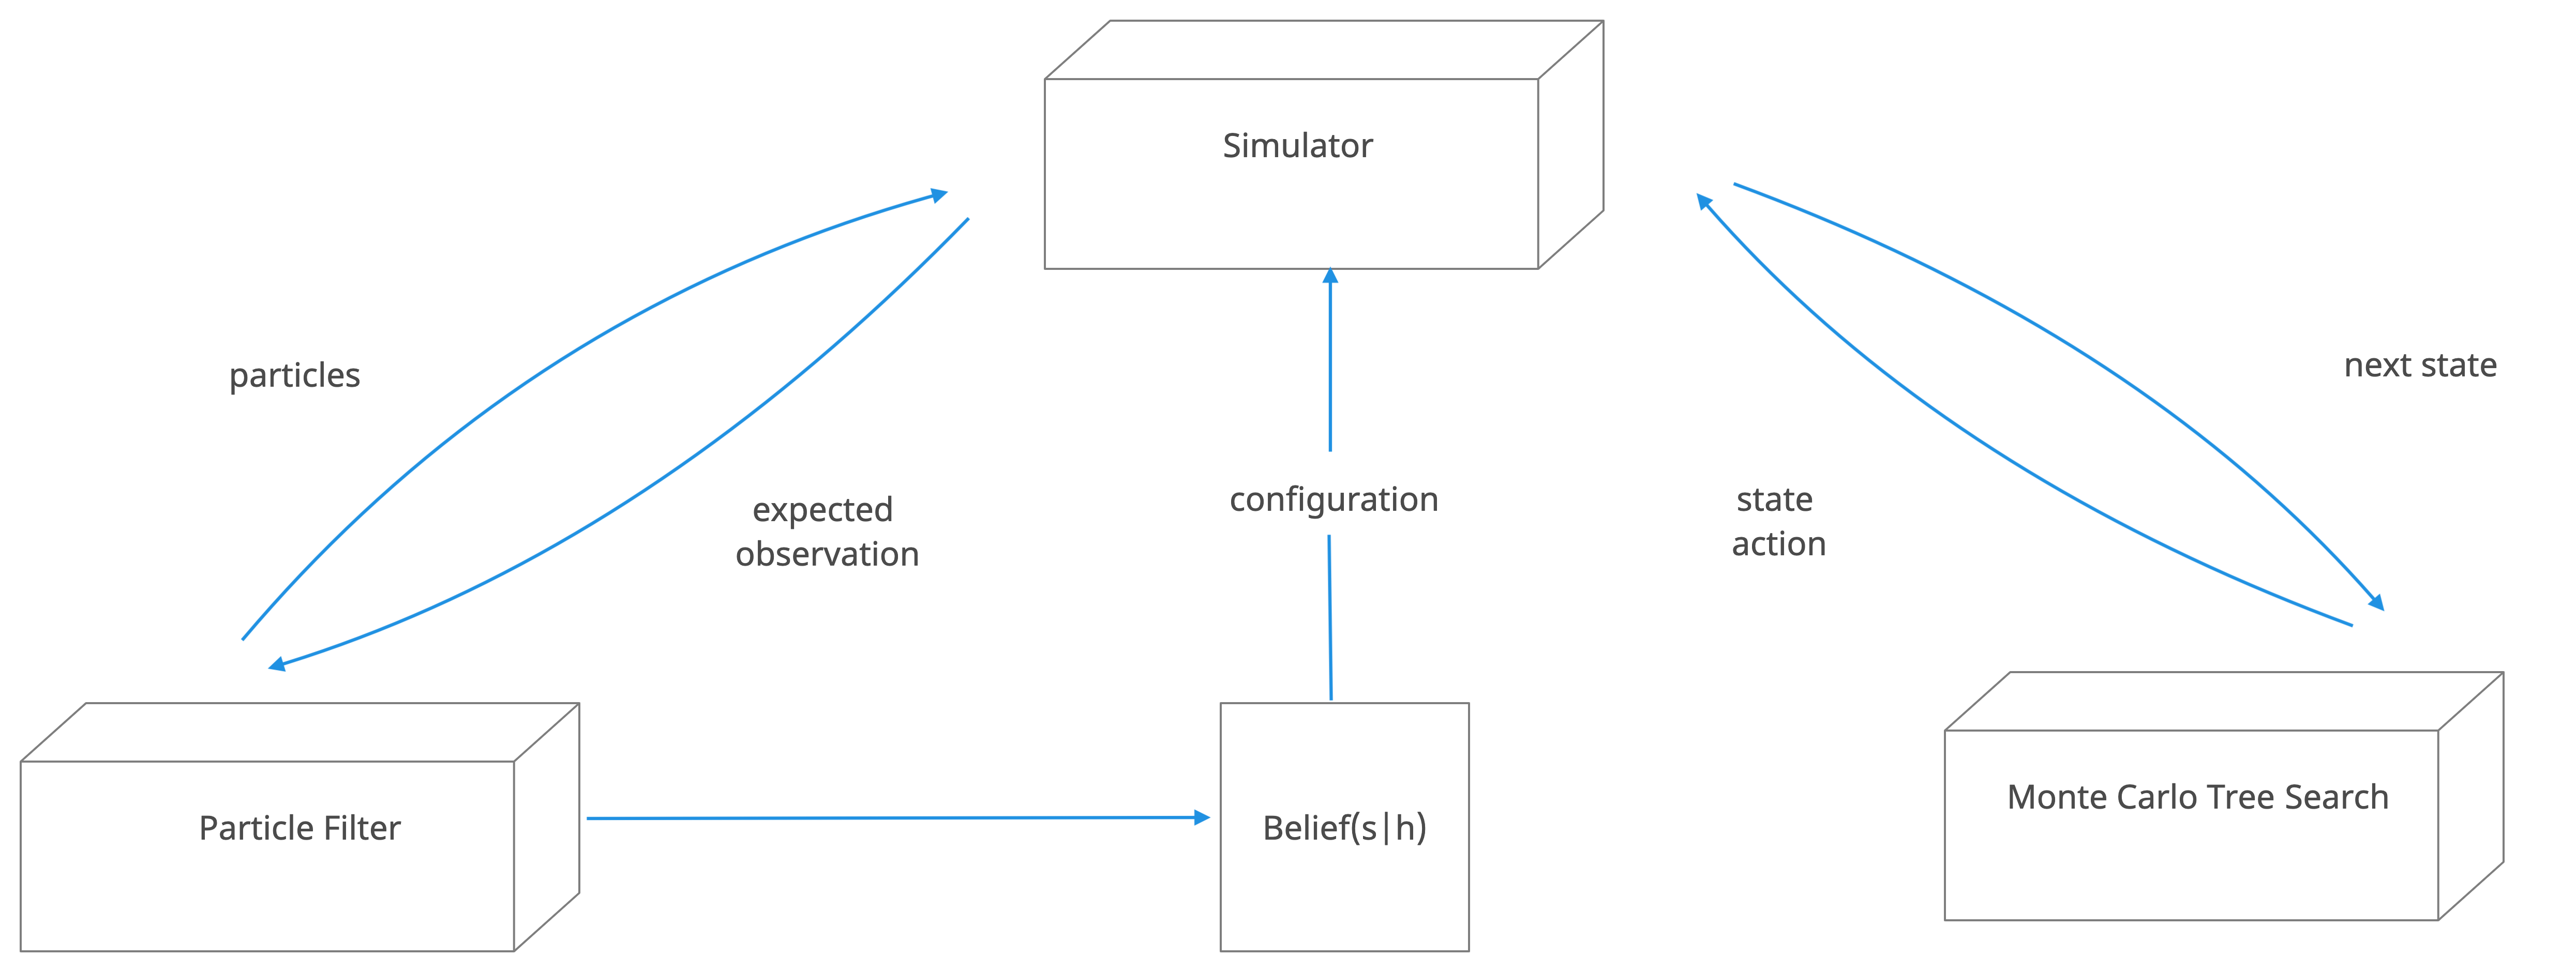
\includegraphics[width=\textwidth]{Figures/POMCP.png}
    \centering  
\end{figure}

As with typical Monte Carlo methods, the sampling approach greatly limits the search space as only (likely) reachable states are evaluated, and the belief over states can be efficiently computed. In short, sampling based methods have shown to allow for swift approximation over complex belief spaces, and the combination of a particle filter with a Monte Carlo Tree Search allows for accurate estimation of the belief-state, and accurate approximation of a near-optimal policy despite complex environments.

\subsubsection{Improving on POMCP --- updating the environment simulation}  
Despite the theoretical success of POMCP, belief-based planning still poses challenges. 
While known for its efficacy in dealing with large state-spaces, MCTS is limited by the accuracy of the transition model. Simply put, if the model of the environment provided to the planner is not sufficiently expressive as to capture the environment dynamics, despite efficient sampling, the performance of an agent will be poor. 
\newline \newline
In recent years, there have been two notable works which have augmented belief-based planners with a learning capacity in order to overcome an incorrectly specified model. 
\newline \newline
Katt et al \cite{Katt2017} augmented the notation of a POMDP to take account of a number of extra features, to allow for a Bayesian updating of the environment model --- in effect the transition dynamics were updated as experience increased in a Bayesian way, allowing for more realistic rollouts and better action selection. In short, they incorportated a learning element into the model of the environment to allow for an incorrectly or incomplete black-box environment simulation. 
\newline \newline
With a similar aim, Hayashi et al \cite{Hayashi_et_al2020} augmented a POMCP planner with a deep-recurrent neural network as a mechanism for particle reinvigoration (suggesting possible states to evaluate), which suggested better candidate states (particles) to be computed allowing noisy or incorrectly specified environments to be used without resulting in poor agent performance. They phrased the environment simulator as a black-box with various parameters which required fitting. This fitting took place as experience grew, meaning that the black-box simulator could be tuned online, allowing the world-model to be iteratively updated. Crucially, they applied this to an opponent modelling task, the level-based foraging domain \cite{Papoudakis2020,Barrett2015}, in which agent types were parameters within the black-box simulator. 

\subsubsection{Incoporating agent models into MCTS}
As mentioned previously, a MCTS involves several stages: 1) traversing a tree via a best-first (heuristic) until reaching a leaf node; 2) Upon reaching a leaf node, it performs a rollout, which involves selecting an action, and sampling an environment simulator for a possible next state and expected reward. It continues this rollout to an arbitrary depth. 3) Finally, having reached a maximum depth, the reward is propagated back up the tree to the root node.
\newline \newline 
In a multi-agent environment, the transition function responsible for mapping one state to another depends on a \textit{joint action} taken by all agents. Hence, in a rollout, the simulator must assume a joint action (i.e. infer/suggest likely actions taken by \textit{other} agents). In this way, agent models are integrated into a MCTS via the simulation phase. In simple terms, they are implicitly included in the environment model --- this is defined mathematically in Section \ref{IncludingAgentModels}. In both \cite{Hayashi_et_al2020} and \cite{Albrecht_stone_2019} agent models are computed and viewed as parameters to be tuned in this environment, thus providing an interesting middle ground between a `global' approach, in which an agent simply learns a single generative model of  the environment from scratch (no opponent models), and a typical opponent modelling approach, which requires distinct agent models and environment models.
\newline \newline
This method also has benefits as it translates the problem of opponent modelling into one of state-space search.

\section{Shortcomings of related/current work}
\subsection{Shortcomings of RL + Search}
The majority of work in the RL + Search space has focused on 2-player zero-sum games. 
This allows for (implicit) opponent modelling via the use of a policy function to guide search: players' intentions are symmetric --- the reward function for a player's opponent is the inverse of that of the player, and as such self-play is a feasible and optimal method of training. 
However, when one moves to a general-sum game (with more than a single opponent), the intentions and characteristics of an opponent are harder to discern, and are likely to vary considerably. Therefore, more explicit and granular representations of a varying/heterogenous opponent types are needed in order to extend this architecture into a general sum, n-player environment.
\newline \newline
RL + Search architectures have focused on well-defined games with perfect observations, and where observations are imperfect all agent actions are public: in effect, all unknowns are known-unknowns, rather than unknown-unknowns. In more fluid games, the adaptation of a partially observable environment cannot always be quite so well translated into public-belief states, and as such, methods like type-based reasoning might still be required despite their relative simplicity and requirement for prior-knowledge.
\subsection{Shortcomings of sample-based planning}
While belief-based planners reason well about agent types, they have failed to adequately address swift action-selection despite having the capacity (and success) of computing a considerable amount of information about opponents. 
In Hayashi et al. \cite{Hayashi_et_al2020}, an opponent model is used solely in the roll-out (black-box simulator/transition simulation) as a predictive model, and not to guide play actively --- action-selection (i.e. tree traversal), and rollout direction is typically guided by a generic upper-confidence tree algorithm.
 The inclusion of a policy network to guide the search tree in an partially observable environment has yet to be truly completed, despite type-based reasoning taking place and being included within the form of parameters for a particle reinvigoration engine. In colloquial terms, information is being computed but not as efficiently and effectively used as it could be.
\newline \newline
Finally, there seems a distinct lack of work regarding actively seeking out information in action-based opponent modelling (N.B. outside of dialogue games). This is somewhat surprising as this area has been identified in several surveys as an open problem, and one worthy of consideration \cite{ALBRECHT201866,Hernandez-Leal_MAL_Survey}. The inclusion of an information theoretic reward (by way of a value function) in an opponent modelling context would be a novel contribution within itself, however it too would be a simple and strong addition to an RL + Search based opponent modelling architecture. 
\newline \newline
In brief: RL+Search architectures have yet to be applied and tested in a multi-agent domain where they must reason about uncertain parameters of opponenet. Belief-based planners have proved to reason well about opponent parameters, however have yet to best leverage learning to shape action-selection despite having shown promise in developing techniques to compute this information.
\section{Opponent specific policy guidance}\label{Contribution}
Previous architectures which have fared well in ad-hoc coordination style environments have applied an agent-policy as opposed to an agent-model \cite{Barrett2015}. This works well with type-based reasoning agents where one can be sure about an agent type, however relies on accurate agent models and a large amount of time to compute them.
\newline \newline
Now, as discussed previously, the purely learned strategies are difficult to be globally accurate, and fail to update swiftly given a new opponent. However, if one has access to an agent type, it stands to reason that one could compute a policy and apply a policy should an agent of that type arrive.
\newline \newline
In recent work, reinforcement learning has been used to restrict the search spaces to only promising moves. The major contribution of this piece of work is to apply opponent-specific policy networks to restrict the search space. Further, the extent of the restriction is dictated by an agent's confidence over the accuracy of an opponent model. Hence, if an opponent is complete unknown, the policy is not used at all, however, should the opponent be similar to an opponent, or similar to two different types of opponent, the search space should be pruned to allow for more searching in areas of the search space which are the most promising for agents of that sort. 
\newline \newline
The generation of these policies relies on offline training of cardinal opponents --- i.e. opponents of a certain sort for a considerable period of time. Given that this policy is subsymbolic, we employ an augmented form of Deep Q learning (dueling Q networks) in order to learn a policy. these networks employ the Bellman equation to provide Q values for all possible actions when given a certain state --- in this case, the observation an agent receives in each timestep.
\subsection{Contribution}
In each timestep, the generative model $G$ used for both the particle filter and for the Monte Carlo Rollouts evaluates particles, and updates the belief-state. In terms of the environment formulation in Section \ref{MDP/POMDP}, it updates the parameters of $\theta$, i.e. the belief over opponent models. For simplicity, the opponent types are limited to four cardinal types --- see appendix for explanation. 
\newline \newline
Having updated the values of $\theta$, the Monte Carlo Search Tree is constructed. The major change from the normal comes in the rollout phase, or specifically, in tayloring the rollouts.
\newline\newline
In each rollout, opponent actions are sampled at random from the set of available moves. In our suggestion, opponent moves are suggested by the opponent model sampled with a distribution computed by the particle filter. By doing this, the joint-action which ultimately dictates the resulting state is, assuming accurate classification of opponents, more accurate. 
\newline \newline
Secondly, during generic Monte Carlo rollouts the agent's actions are selected at random from the set of all agent's possible actions. In our modification, the agent's actions are sampled based on the probability of certain opponents, from the policies corresponding to those opponents. Therefore further pruning the samples to explore the search space which is likely to be the most promising. 
\newline\newline
We suggest that this is the first attempt in the field to have employed opponent-weighted policies to prune a search space for a fundamentally model-based agent. 

\section{Experimental Evaluation}

\subsection{Ad-hoc coordination: a challenge}
A large proportion of opponent modelling research has been directed at adversarial games. 
This allows a number of assumptions to be made about opposing agents (hence the name `opponent' modelling). The major assumption made is that of a purely adversarial opponent. From this assumption, one can assume that the reward function of an opposing agent is the inverse of their own. Given the assumption of an opponents reward function (or at a higher level, their intentions), one can employ a number of techniques to optimise actions --- for instance, pre-computing equilibria via iterative methods (e.g. fictitous play), self-play (training against oneself) and minimax pruning. These techniques have been used well previously in zero-sum games like Poker, Go and Chess. When one extends to environments which require cooperation as well as coompetetive objectives, these techniques require modification to be applicable. 
\newline \newline
The major effort behind this line of work is to extend opponent modelling techniques to more general problems, or more specifically, open environments. A growing field of research investigates ad-hoc coordination games. These are typically games which are sufficiently simple to be computed by an agent with limited computational power, but incorporate sufficient complexity as to be challenging. Rather more importantly, these games involve self-interested agents (i.e. no common world-model or shared objectives) and allow for competetive agents, however often require cooperation to acheive optimal results. They often involve more than a single other agent, and those other agents often can be deliberatly adversarial or cooperative in nature.
\newline \newline 
This environment shares a number of aspects with open domains: a number of heterogenous agents, exhibiting a variety of intents and abilities in a partially observable (uncertain) environment. Hence, this serves as a strong test-bed for an opponent modelling system designed for an open system and provides a number of state of the art systems to augment and benchmark against. 
\subsubsection{The level-based foraging domain}
A plausible environment (among a number of others) are variations of the Level-based foraging domain (LBFD) (used by \cite{Albrecht2019,Barrett2015,Hayashi_et_al2020,Papoudakis2020}\footnote{This is not an exhaustive list.}). The LBFD is represented by a two dimensional gridworld with a number of self-interested agents.
The gridworld is populated by agents and objects. Each agent and object has a \textit{level}. The game finishes after an arbitrary number of timesteps, or when all objects have been foraged. Agents have 6 discrete actions in each timestep :(north, south, east, west, stay still, load block). All agents more asynchronously, and select a single action per timestep. Agents receive a reward for foraging an object equal to the object's level. Agents cannot forage any object with a higher level than their own. In the case where an object's level is higher than an agent, agents can cooperate in order to forage the object together, providing that the sum of their levels' is greater than that of the object.  
\subsection{Baselines in ad-hoc coordination}
\begin{enumerate}
    \item Plastic Policy \cite{Barrett2015} \newline \newline
Barrett et al. make a key contribution: they learn an optimal policy for acting with teammates in a simulated robo-soccer league via fitted q learning. They argue that in a complex domain it is necessary to move from a model-based approach to a policy-based approach due to prohibitively large state-spaces. At runtime they select which policy to use by a nearest neighbour classification based on action histories. This contains no feature of learning at runtime and assumes that the types are sufficiently expressive, and that the policies are optimal. Hence, when exposed to unknown agents, this \textit{should}, in theory, perform worse than methods which have internal parameters to update. 
    \item Albrecht and Stone: reasoning about uncertain agent parameters\cite{Albrecht_stone_2019}.  \newline \newline
Barrett and Stone addressed the problem of static types by including parameters within agent types, and perform an element of policy reconstruction within type-based reasoning. They suggest 3 methods of updating parameter values (approximate gradient ascent, approximate bayesian updating, and exact global updating) and provide a heuristic for selectively updating type's parameters. They then use a MCTS algorithm to evalute the best action. 
\item Hayashi et al --- Particle filtering with DRNNs \cite{Hayashi_et_al2020}. \newline \newline
Hayashi et al. employ type-based reasoning with parameterisation. They encorporate the opponent types and parameters within types into the black-box environment simulator for the POMCP. They then select optimal actions via a MCTS planner at run-time. Their contribution, a deep-recurrent neural network architecture for particle reinvigoration, shows to perform well at updating despite an initially poorly configured model. At runtime, they use an unspecified heuristic for rollout policy. 
\end{enumerate}
Both Hayashi et al and Albrecht and Stone focus on inferring a correctly specified world model, and query this world model with a MCTS style algorithm. However, unlikey Barrett et al, they do not update their actions given this information, and rely solely on the MCTS to adapt, given the inclusion of the opponent model in the rollouts. Given that the existence of types imples an element of prior knowledge, it seems only reasonable to update actions, even if it is only to direct the rollouts, given this information, as opposed to an entire prior-learned policy.  
\subsection{Experiments}
\begin{itemize}
    \item Baseline --- plastic policy
    \item Baseline --- Monte Carlo Agent
    \item Baseline --- Monte Carlo Particle Filter
    \item Show average performance against randomly selected opponents over 10000 rounds. 
    \item Show 
    \item Monte Carlo Policy --- show robustness to reduced sample/rollout size. 
    \item Show robustness compared to learning agent (in terms of learning)
\end{itemize}
\subsection{Evaluation/Thoughts}
\section{Future work \& Conclusions}
\begin{itemize}
    \item Monte Carlo --- supervised learning for quick learning and policy generation (Similar to monte-carlo A3C supervision...)
    \item Value theoretic function --- learn more about opponents to better classify faster
    \item Strategy Generation --- Monte Carlo agent for strategy imposing... 
\end{itemize}
\subsection{Closing comments}

\bibliographystyle{aaai}  
\bibliography{library.bib}
\appendix
\section{Opponent Types description}
\section{Policy learning hyperparameters}
\section{Proof of convergence for MCTS and PF}


\end{document}